%LTeX: language=it
<<<<<<< HEAD
\subsection{UC 6 - Creazione di una cartella} \label{sec:UC6}
    \begin{itemize}
        \item \textbf{Attore principale}: MUA;
        \item \textbf{Descrizione}: il MUA crea una cartella nel sistema;
        \item \textbf{Precondizioni}: il MUA sta usando la funzionalità di creazione di un oggetto;
        \item \textbf{Postcondizioni}: il sistema salva la nuova cartella creata;
        \item \textbf{Scenario principale}:
            \begin{enumerate}
                \item il MUA invia le informazioni per creare la cartella (\hyperref[sec:UC6.1]{UC 6.1});
                \item il sistema salva la nuova cartella;
            \end{enumerate}
        \item \textbf{Inclusioni}: nessuna;
        \item \textbf{Generalizzazioni}: nessuna;
        \item \textbf{Estensioni}: nessuna.
    \end{itemize}

\begin{figure}[h]
    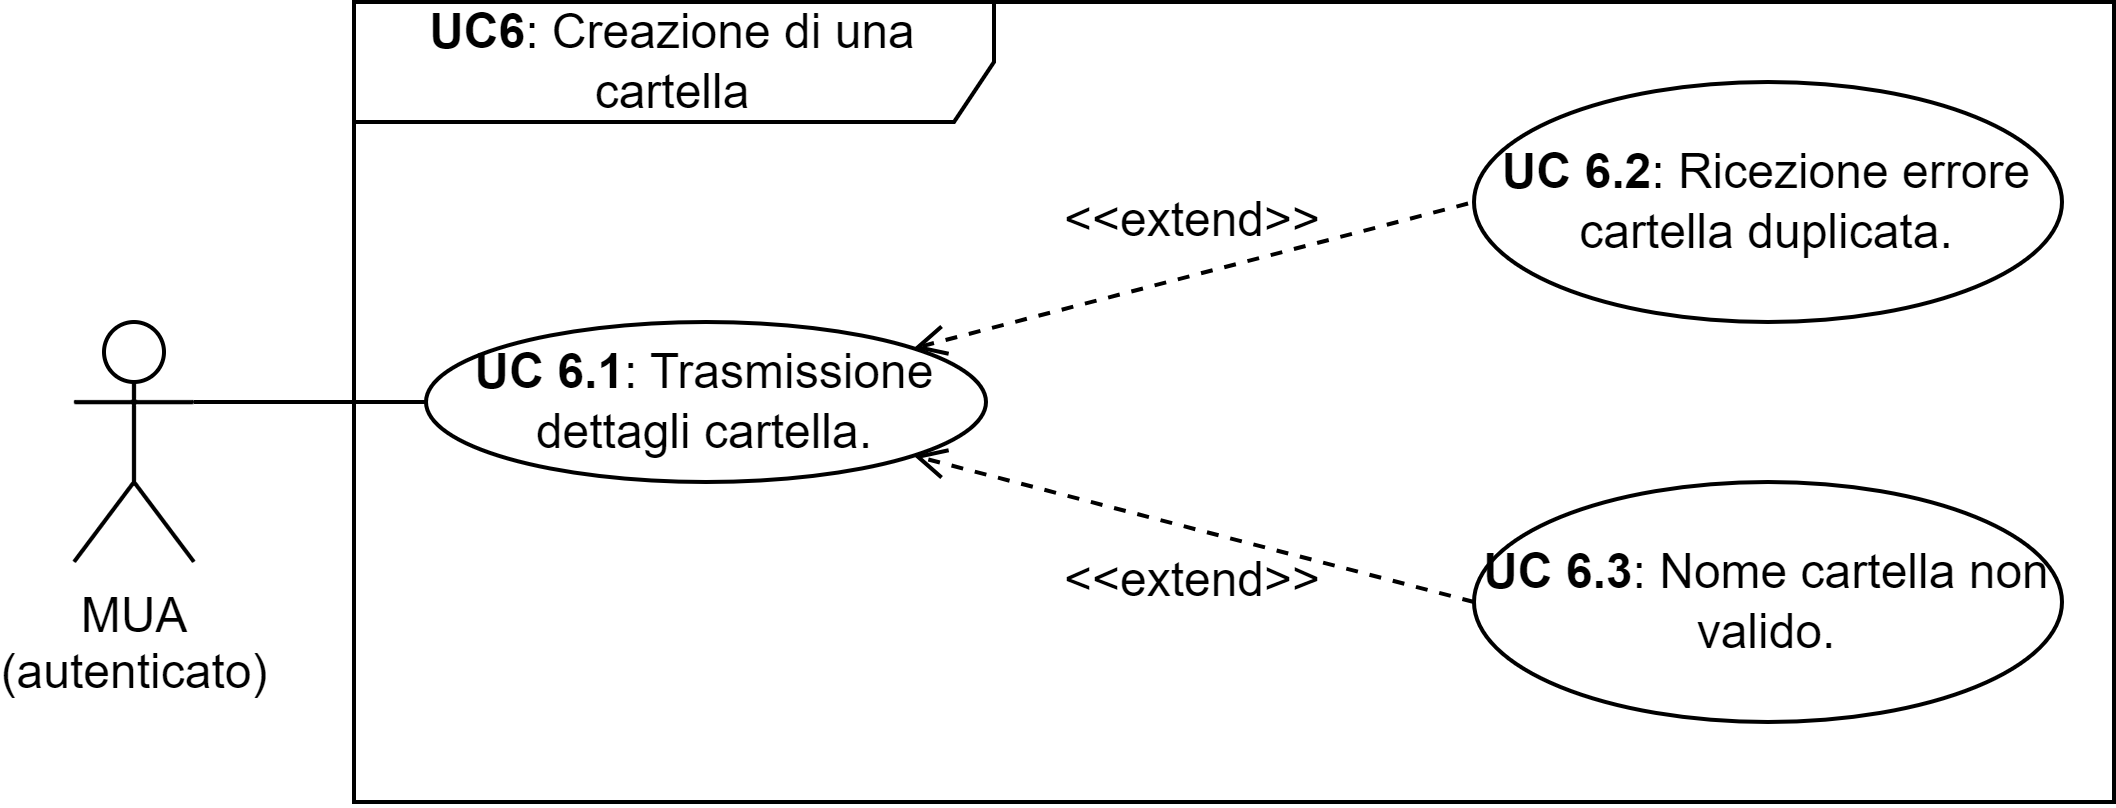
\includegraphics[width=0.85\textwidth]{sections/uc_imgs/UC06.X.png}
    \centering
    \caption{Diagramma sotto-casi UC 6.}
\end{figure}

\subsubsection{UC 6.1 - Trasmette dettagli della cartella} \label{sec:UC6.1}
    \begin{itemize}
        \item \textbf{Attore principale}: MUA;
        \item \textbf{Descrizione}: il MUA trasmette i dettagli per creare la cartella al sistema;
        \item \textbf{Precondizioni}: il MUA sta usando la funzionalità di creazione di una cartella;
        \item \textbf{Postcondizioni}: il sistema salva la nuova cartella creata;
        \item \textbf{Scenario principale}:
            \begin{enumerate}
                \item il MUA invia le informazioni necessarie per creare la cartella;
                \item il sistema elabora le informazioni ricevute, controlla che:
                \begin{itemize}
                    \item il nome ricevuto non è una stringa vuota;
                    \item che il path indicato sia valido;
                \end{itemize}
            \end{enumerate}
        \item \textbf{Inclusioni}: nessuna;
        \item \textbf{Generalizzazioni}: nessuna;
        \item \textbf{Estensioni}:
            \begin{enumerate}[label=\alph*.]
                \item il sistema non riesce a salvare la cartella perché è un duplicato:
                \begin{enumerate}[label=\arabic*.]
                    \item il sistema ritorna un errore al MUA di cartella duplicata (\hyperref[sec:UC6.2]{UC 6.2});
                \end{enumerate}
                \item il sistema non riesce a creare la cartella perché i dettagli forniti non sono validi:
                \begin{enumerate}[label=\arabic*.]
                    \item il sistema ritorna un errore al MUA dove lo informa che i dettagli forniti non sono validi(\hyperref[sec:UC6.3]{UC 6.3}).
                \end{enumerate}
            \end{enumerate}
    \end{itemize}

\subsubsection{UC 6.2 - Ritorna l'errore cartella duplicata} \label{sec:UC6.2}
    \begin{itemize}
        \item \textbf{Attore principale}: MUA;
        \item \textbf{Descrizione}: il MUA trasmette i dettagli per creare la cartella al sistema;
        \item \textbf{Precondizioni}: il MUA sta trasmettendo le istruzioni per la creazione di una cartella;
        \item \textbf{Postcondizioni}: il sistema non crea la nuova cartella e il MUA viene notificato dell'errore;
        \item \textbf{Scenario principale}:
            \begin{enumerate}
                \item il sistema nota che la cartella esiste già e annulla l'operazione per la creazione della cartella;
                \item il sistema notifica l'utente dell'errore;
            \end{enumerate}
        \item \textbf{Inclusioni}: nessuna;
        \item \textbf{Generalizzazioni}: nessuna;
        \item \textbf{Estensioni}: nessuna.
    \end{itemize}

    \subsubsection{UC 6.3 - Ritorna l'errore dettagli non validi} \label{sec:UC6.3}
    \begin{itemize}
        \item \textbf{Attore principale}: MUA;
        \item \textbf{Descrizione}: il MUA trasmette i dettagli per creare la cartella al sistema;
        \item \textbf{Precondizioni}: il MUA sta trasmettendo le istruzioni per la creazione di una cartella;
        \item \textbf{Postcondizioni}: il sistema non crea la nuova cartella e il MUA viene notificato dell'errore;
        \item \textbf{Scenario principale}:
            \begin{enumerate}
                \item il sistema i dettagli non rispettano i requisiti richiesti e annulla l'operazione per la creazione della cartella;
                \item il sistema notifica l'utente dell'errore;
            \end{enumerate}
        \item \textbf{Inclusioni}: nessuna;
        \item \textbf{Generalizzazioni}: nessuna;
        \item \textbf{Estensioni}: nessuna.
    \end{itemize}
=======
\subsection{UC 6 - Creazione condivisione} \label{sec:UC6}
    \begin{itemize}
        \item \textbf{Attore principale}: MUA;
        \item \textbf{Descrizione}: il MUA deve poter creare una condivisione nel sistema;
        \item \textbf{Precondizioni}: l’account che il MUA gestisce è registrato nel sistema, ha una connessione aperta con il sistema ed è autenticato;
        \item \textbf{Postcondizioni}: il MUA crea una condivisione che viene salvata nel sistema;
        \item \textbf{Scenario principale}:
        \begin{enumerate}
            \item il MUA invia la condivisione al sistema;
            \item il sistema salva la condivisione;
        \end{enumerate}
    \item \textbf{Inclusioni}: nessuna;
    \item \textbf{Generalizzazioni}:
        \begin{itemize}
            \item il MUA crea una condivisione di una cartella (\hyperref[sec:UC7]{UC 7});
            \item il MUA crea una condivisione di un contatto (\hyperref[sec:UC8]{UC 8});
            \item il MUA crea una condivisione di un evento (\hyperref[sec:UC9]{UC 9});
        \end{itemize}
    \item \textbf{Estensioni}: nessuna;
\end{itemize}
>>>>>>> 177cc19041165c8485927b56b5ea094ec2cbcfb6
